\section{Reštiev}
Najprej narišemo funkciji $\Ai$ in $\Bi$ z uporabo builtin funkcij v
knjižnjici \verb|mpmath| in \verb|matplotlib|.

\begin{figure}[h]
    \begin{center}
        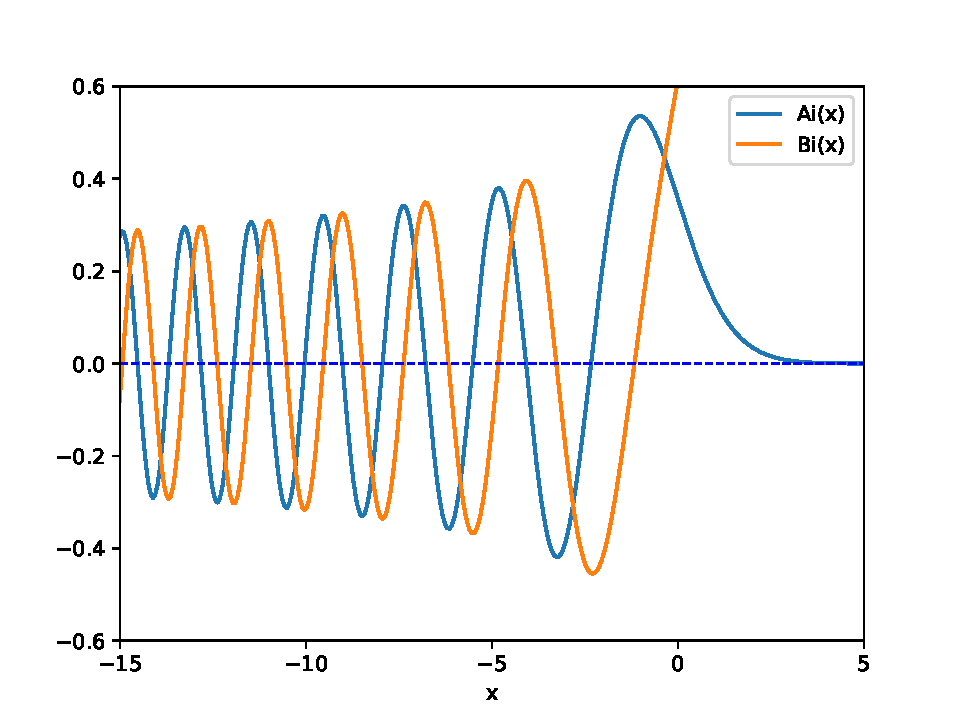
\includegraphics[width=13cm]{sections/poglavje1/pdfs/True_airy.pdf}
        \caption{Funkciji $\Ai(x)$ in $\Bi(x)$}
        \label{slika 1}
    \end{center}
\end{figure}

Nato sem risal za majhne $x$ s pomočjo razvojem $\Ai$ ter $\Bi$
v Maclaurinovo vrsto.

\begin{equation}
    \Ai(x) = \alpha f(x) - \beta g(x)\>,\qquad
    \Bi(x) = \sqrt{3}\, \Bigl[\alpha f (x) + \beta g(x) \Bigr]\>,
\end{equation}
kjer v $x=0$ veljata zvezi
%
$\alpha = \Ai(0) = \Bi(0)/\sqrt{3}\approx 0.355028053887817239$ in
$\beta = -\Ai'(0) = \Bi'(0)/\sqrt{3}\approx 0.258819403792806798$.
Vrsti za $f$ in $g$ sta
\begin{equation}
  f(x) = \sum_{k=0}^\infty
  \left(\frac{1}{3}\right)_k \frac{3^k x^{3k}}{(3k)!} \>, \qquad
  g(x) = \sum_{k=0}^\infty
  \left(\frac{2}{3}\right)_k \frac{3^k x^{3k+1}}{(3k+1)!} \>,\label{2}
\end{equation}
kjer je
\begin{equation}
  (z)_k = \Gamma(z+k)/\Gamma(z) \>, \qquad (z)_0 = 1 \>.\label{3}
\end{equation}

Enačbo \eqref{3} lahko še naprej razpišemo.
\begin{equation}
    \Gamma(z+k)/\Gamma(z) = \frac{(z+k-1)!}{(z-1)!}\label{4}
\end{equation}
Fakulteta za necela števila za večja od $1$, velja isto rekurzivno
pravilo kot za cela števila. Za števila med $0$ in $1$ se fakulteto izračuna numerično.
Tako potreubujemo vrednosti:
\begin{equation}
    \left(\frac{1}{3}\right)! \;=\;\Gamma(4/3) \;=\; 0.89297951156924921
\end{equation}
\begin{equation}
    \left(\frac{2}{3}\right)! \;=\;\Gamma(5/3) \;=\; 0.90274529295093361
\end{equation}

Vstavimo dobljeno \eqref{4} v sumand \eqref{2}.
\begin{equation}
    f(x) = 1+\sum_{k=1}^{\infty}\frac{1}{3}\frac{(\frac{1}{3}+k-1)!}{\left(\frac{1}{3}\right)!}
    \frac{3^k x^{3k}}{(3k)!} = 1+\frac{1}{3\left(\frac{1}{3}\right)!}\sum_{k=1}^{\infty}(\frac{1}{3}+k-1)!\frac{3^k x^{3k}}{(3k)!}
\end{equation}
Na zvit način se pa jih znebimo, če še naračunamo do $k=1$, namreč $\left(\frac{1}{3}\right)!$ se pokrajša. Podobno naredimo za funkcijo $g(x)$.
Graf funkcije dobimo in izgleda takole:
\begin{figure}[h]
    \begin{center}
        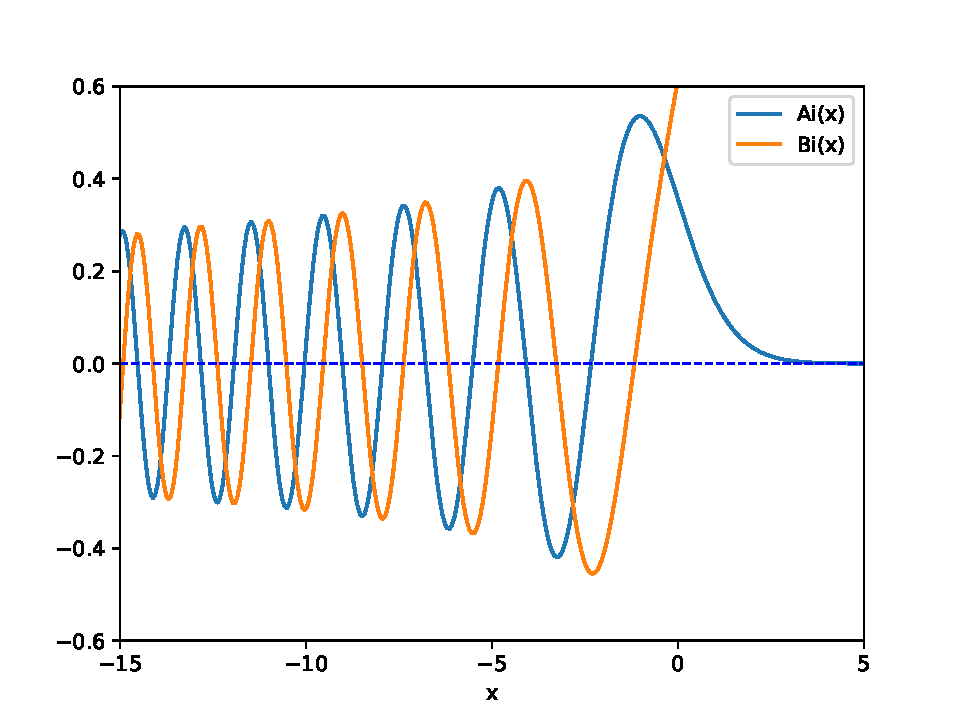
\includegraphics[width=13cm]{sections/poglavje1/pdfs/small_airy.pdf}
        \caption{Funkciji $\Ai(x)$ in $\Bi(x)$ razviti po taylorju}
        \label{slika 2}
    \end{center}
\end{figure}

Za velike vrednosti $|x|$ Airyjevi funkciji aproksimiramo
z njunima asimp\-tot\-ski\-ma razvojema.  Z novo spremenljivko
$\xi=\frac{2}{3} |x|^{3/2}$ in asimptotskimi vrstami
%
\begin{equation}
  L(z) \sim \sum_{s=0}^\infty \frac{u_s}{z^s}\>,\qquad
  P(z) \sim \sum_{s=0}^\infty (-1)^s \frac{u_{2s}}{z^{2 s}}\>,\qquad
  Q(z) \sim \sum_{s=0}^\infty (-1)^s \frac{u_{2s+1}}{z^{2 s+1}}\>,
\end{equation}
s koeficienti
\begin{equation}
u_s = \frac{ \Gamma(3s + \frac{1}{2})}
        {54^s s!\, \Gamma(s + \frac{1}{2}) } \label{9}
\end{equation}
za velike pozitivne $x$ izrazimo
%
\begin{equation}
\Ai(x)\sim  \frac{\mathrm{e}^{-\xi}}{2\sqrt{\pi} x^{1/4}} \, L(-\xi) \>, \qquad
\Bi(x)\sim  \frac{\mathrm{e}^{\xi}} { \sqrt{\pi} x^{1/4}} \, L(\xi)\>,
\end{equation}
%
za po absolutni vrednosti velike negativne $x$ pa
%
%
\begin{align}
    \Ai(x)&\sim  \frac{1}{\sqrt{\pi} (-x)^{1/4}}
    \Bigl[ \phantom{-}\sin(\xi-\pi/4) \, Q(\xi)
                    + \cos(\xi-\pi/4) \, P(\xi)\Bigr] \>, \\
    \Bi(x)&\sim  \frac{1}{\sqrt{\pi} (-x)^{1/4}}
    \Bigl[ - \sin(\xi-\pi/4) \, P(\xi)
      + \cos(\xi-\pi/4) \, Q(\xi)\Bigr]\>.
\end{align}

Koeficiente \eqref{9} lahko izrazimo:
\begin{equation}
    \frac{\Gamma(3s+\frac{1}{2})}{\Gamma(s+\frac{1}{2})} = \frac{(3s-\frac{1}{2})!}{(s-\frac{1}{2})!}
\end{equation}
Dobimo naslednjo sliko za asimptotski približek funkciji.
\newpage
\begin{figure}[h]
    \begin{center}
        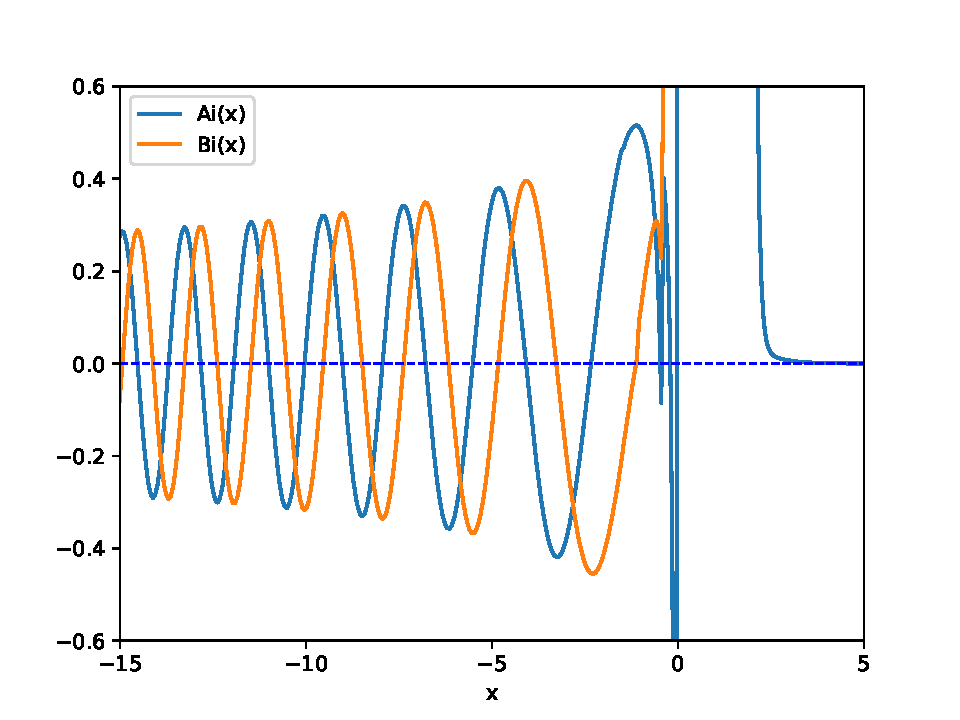
\includegraphics[width=13cm]{sections/poglavje1/pdfs/big_airy.pdf}
        \caption{Funkciji $\Ai(x)$ in $\Bi(x)$ asimptotsko razvit}
        \label{slika 3}
    \end{center}
\end{figure}\
\newpage
Iz samega grafa ne vidimo odstopanja od prave vrednosti, zato si poglejmo absolutno napako in relativno.

\begin{figure}[h]
    \begin{center}
        \subfigure[Absolutna napaka]{
            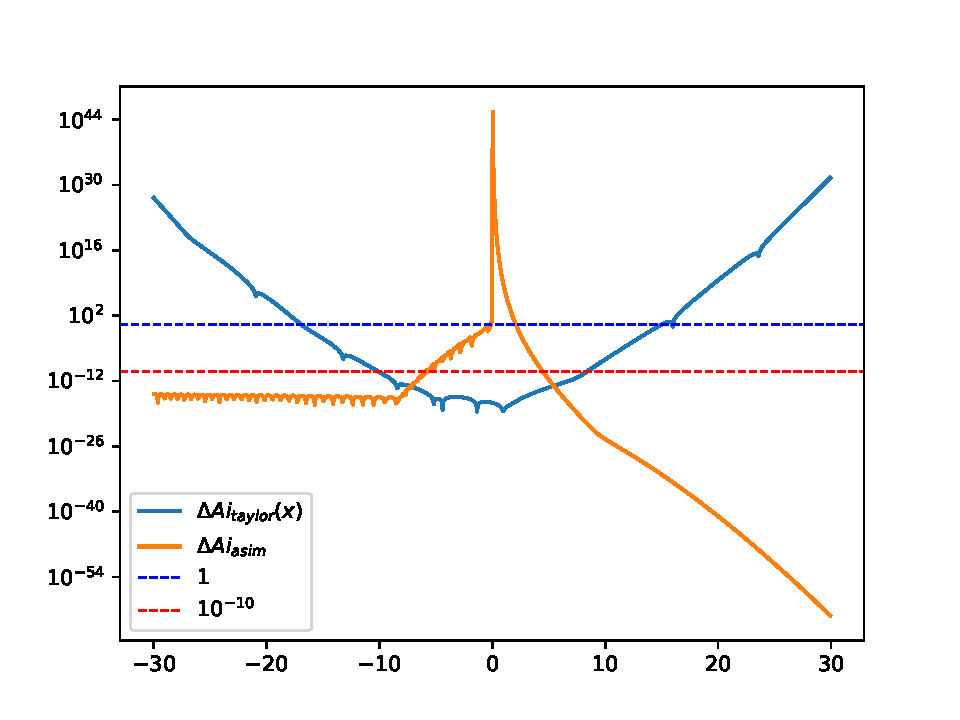
\includegraphics[width=9cm]{sections/poglavje1/pdfs/Ai_abs_error.pdf}
        }
        \subfigure[Relativna napaka]{
            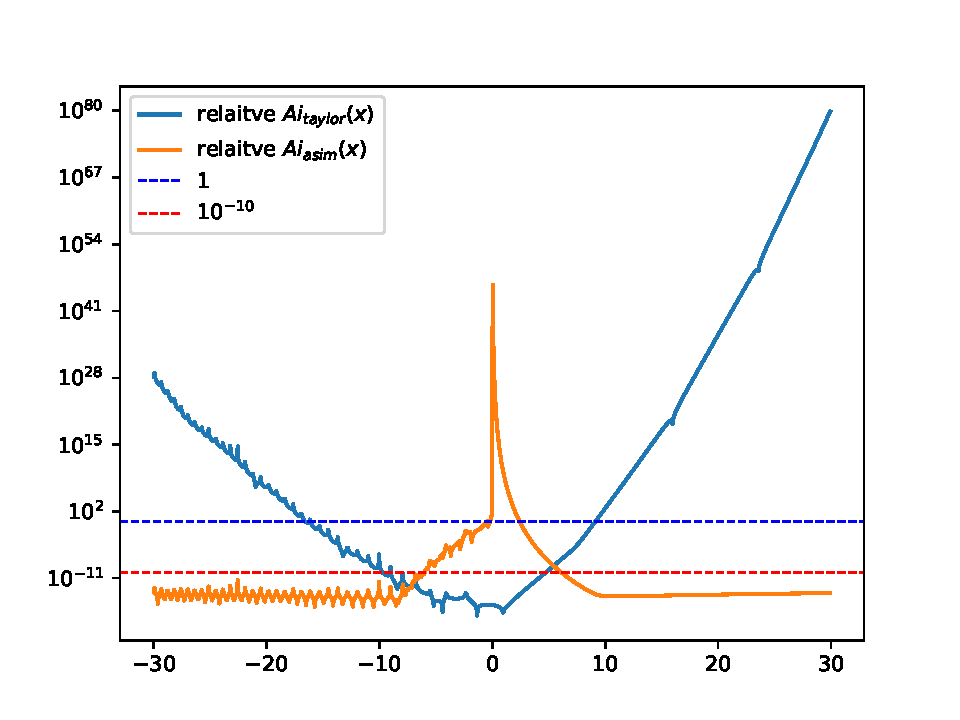
\includegraphics[width=9cm]{sections/poglavje1/pdfs/Ai_rel_error.pdf}
        }
        \caption{Funkcija $\Ai(x)$ absolutna in relativna napaka}
        \label{slika 4}
    \end{center}
\end{figure}
Kar zadošča nalogi na intervalu $x \in \left[-\infty,\; 8 \right]$. Poglejmo si še za funckijo $\Bi(x)$.
\newpage
\begin{figure}[h]
    \begin{center}
        \subfigure[Absolutna napaka]{
            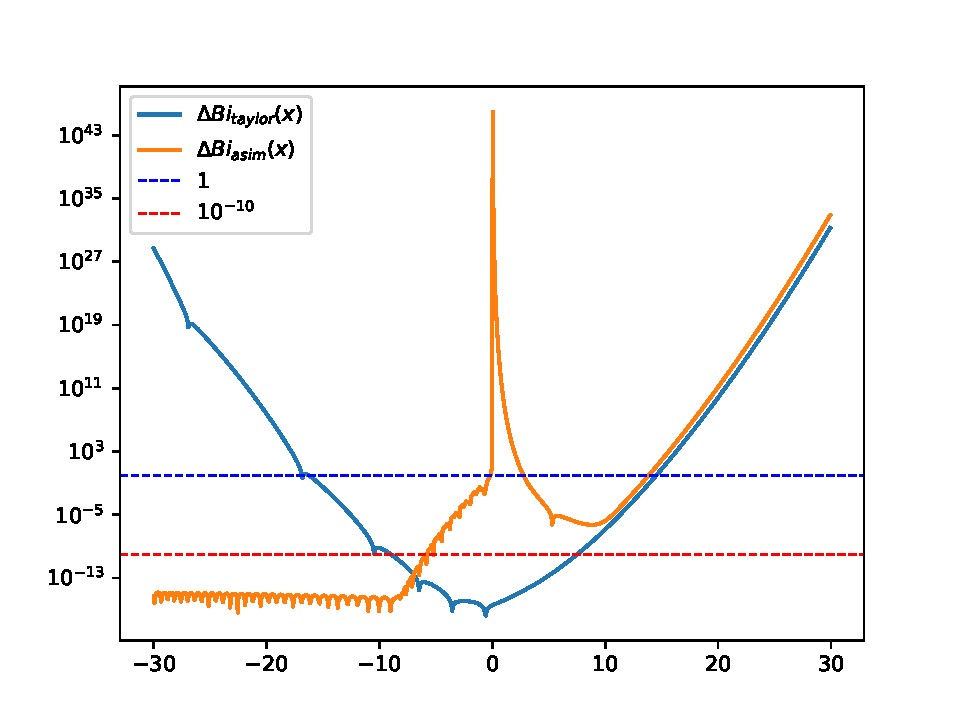
\includegraphics[width=9cm]{sections/poglavje1/pdfs/Bi_abs_error.pdf}
        }
        \subfigure[Relativna napaka]{
            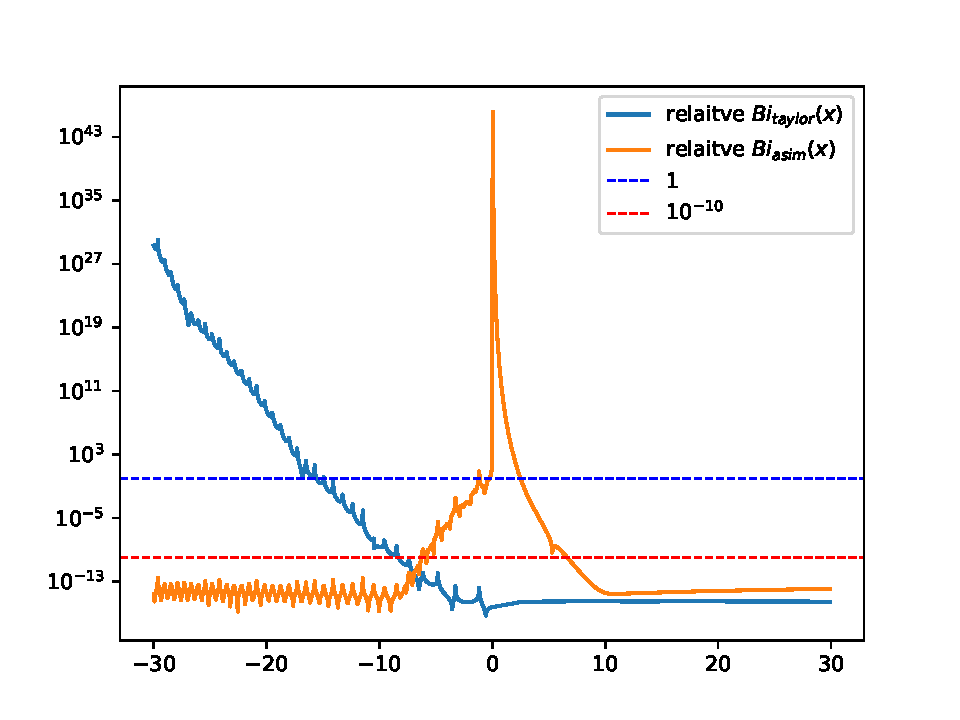
\includegraphics[width=9cm]{sections/poglavje1/pdfs/Bi_rel_error.pdf}
        }
        \caption{Funkcija $\Bi(x)$ absolutna in relativna napaka}
        \label{slika 5}
    \end{center}
\end{figure}